\documentclass[aspectratio=169]{beamer}
\usepackage{beamerthemesplit}
\usepackage{multirow}
\usepackage{array}
\usepackage{hyperref}
\usepackage[T1]{fontenc}
\usepackage{inconsolata}
\usepackage{xcolor,colortbl}
\usepackage{natbib}
\usepackage{listings}
%%\newcommand{\newblock}{}
\DeclareGraphicsExtensions{.pdf,.png,.jpg}
\usetheme[pageofpages=of,% String used between the current page and the
                         % total page count.
          bullet=circle,% Use circles instead of squares for bullets.
          titleline=true,% Show a line below the frame title.
          alternativetitlepage=true,% Use the fancy title page.
          ]{Torino}
\definecolor{light-green}{RGB}{144,238,144}
\makeatletter
\setbeamertemplate{footline}
{
  \leavevmode%
  \hbox{%
  \begin{beamercolorbox}[wd=.333333\paperwidth,ht=2.25ex,dp=1ex,center]{author in head/foot}%
    \usebeamerfont{author in head/foot}\insertshortauthor~~\beamer@ifempty{\insertshortinstitute}{}{(\insertshortinstitute)}
  \end{beamercolorbox}%
  \begin{beamercolorbox}[wd=.333333\paperwidth,ht=2.25ex,dp=1ex,center]{title in head/foot}%
    \usebeamerfont{title in head/foot}\insertshorttitle
  \end{beamercolorbox}%
  \begin{beamercolorbox}[wd=.333333\paperwidth,ht=2.25ex,dp=1ex,right]{date in head/foot}%
    \usebeamerfont{date in head/foot}\insertshortdate{}\hspace*{2em}
%    \insertframenumber{} / \inserttotalframenumber\hspace*{2ex} % DELETED
  \end{beamercolorbox}}%
  \vskip0pt%
}
\makeatother
\begin{document}
\author{{\bf Casey Stella}\\@casey\_stella}
\institute[Hortonworks]{
\includegraphics[width=40px,height=17px]{logo}}
\title{{\bf Apache Metron }}
\subtitle{{\bf A Case Study of a Modern Streaming Architecture on Hadoop}}
\date{2017} 

\frame{\titlepage} 

\begingroup
\Huge
\begin{frame}
\frametitle{Introduction}
\begin{center}
Hi, I'm Casey Stella!
\end{center}
\end{frame}
\endgroup

\section{Apache Metron}

\frame{\frametitle{Apache Metron: A Cybersecurity Analytics Platform}
\begin{itemize}
\item Metron provides a scalable, advanced security analytics framework to offer a centralized tool for security monitoring and analysis.
\item Metron was initiated at Cisco in 2014 as OpenSOC.
\item Metron was submitted to the Apache Incubator in December 2015
\item Metron graduated to a top level project in April 2017
\end{itemize}
}

\frame{\frametitle{Characteristics of Metron}
\begin{itemize}
\item Metron is built atop the Apache Hadoop ecosystem handle capturing, ingesting, enriching and storing streaming data at scale
  \begin{itemize}
  \item Kafka provides a unified data bus
  \item Storm providing a distributed streaming framework
  \item HBase provides a low latency key/value lookup store for enrichments and profiles
  \item Zookeeper provides a distributed configuration store
  \end{itemize}
\item Ingested network telemetry can be enriched pluggably
  \begin{itemize}
  \item New enrichments can be done live on running topologies without restart
  \item New enrichment capabilities can be added via user defined functions
  \item Enrichments can be composed through a domain specific language called {\bf Stellar}
  \end{itemize}
\item Data stored in HBase can be the source of enrichments
\end{itemize}
}

\frame{\frametitle{Characteristics of Metron}
\begin{itemize}
\item Enriched network telemetry can be indexed into a Security data lake
  \begin{itemize}
  \item Indexes supported are pluggable and include HDFS, Solr and Elasticsearch
  \end{itemize}
\item Advanced analytics can be done on streaming data
  \begin{itemize}
  \item Probabalistic data structures (e.g. sketches) can sketch streaming data across time and enable approximate distribution, set existence and distinct count queries
  \item Models can be deployed using Yarn, autodiscovered via Zookeeper and interrogated via Stellar functions
  \end{itemize}
\end{itemize}
}

\frame{\frametitle{Stellar}
Metron needed the ability to allow users to pluggably and consistently enrich and transform streaming data.
Out of this need, we created {\bf Stellar}: 
\begin{itemize}
\item Interact with the various enabling Hadoop components in a unified manner
\item Compose a rich set of built-in functions with user defined functions
\item Provide simple primitives around the functions: boolean operations, conditionals, numerical computation.
\end{itemize}
Think of Stellar as similar to Excel functions that we can run on streaming data.
}



\frame{\frametitle{Data Ingest: Parsers}
\begin{itemize}
\item Telemetry data comes in a variety of formats and velocities.
\item Each telemetry source is ingested into kafka
\item A Storm {\bf parser} topology is used to convert the raw telemetry format to a normalized JSON Map
  \begin{itemize}
  \item Common network-related raw telemetry formats 
  \item Specifying the parser via Grok
  \item Generic formats such as CSV and JSON 
  \item Creating your own parser in a JVM-based language
  \end{itemize}
\item Simple transformations and normalizations can be done post-parse via Stellar statements
\item The normalized data across all telemetries is written to an {\bf enrichment} kafka topic
\end{itemize}
}

\frame{\frametitle{Data Ingest: Parsers}
\begin{center}
  \makebox[\textwidth]{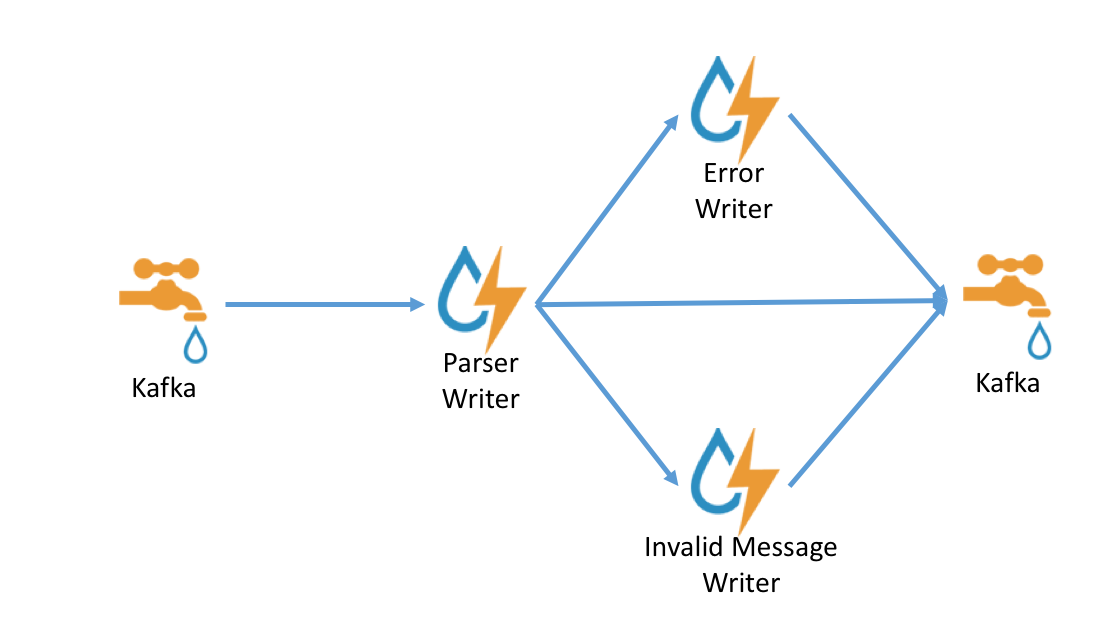
\includegraphics[scale=0.4]{images/parser_arch.png}}
\end{center}
}

\frame{\frametitle{Enrichment}
\begin{itemize}
\item The enrichment topology takes the various normalized telemetry sources and allows users to enrich the messages with broader context
  \begin{itemize}
  \item Enriching with reference data ingested into HBase
  \item Enriching via arbitrary Stellar expressions
  \item Enriching with Geolocation data
  \end{itemize}
\item Enrichment is split into two phases
  \begin{itemize}
  \item Preparatory Enrichment
  \item Threat Intelligence Enrichment
  \end{itemize}
\item If messages are marked with an {\bf is\_alert} field, they can have a triage score computed via Stellar which defines their priority as threats
\end{itemize}
}

\frame{\frametitle{Enrichment: HBase}
A core enrichment source is enriching messages with reference data stored in HBase.  
Metron provides a loading framework which takes data and
\begin{itemize}
\item Defines a logical key for the HBase enrichment via Stellar
\item Loads the data into HBase via MapReduce or directly depending on data size
\item For reference data which is streamed in, you can write to HBase from a parser and ingest the streaming reference data as any other telemetry
\end{itemize}
}

\frame{\frametitle{Enrichment: Stellar}
Stellar is the primary method for enrichment in Metron.  
\begin{itemize}
\item User defined enrichment functions can be enabled through adding a jar implementing the function to HDFS.
\item Stellar enrichments can be executed asynchronously across storm workers and their results joined together
\end{itemize}
}

\frame{\frametitle{Enrichment}
\begin{center}
  \makebox[\textwidth]{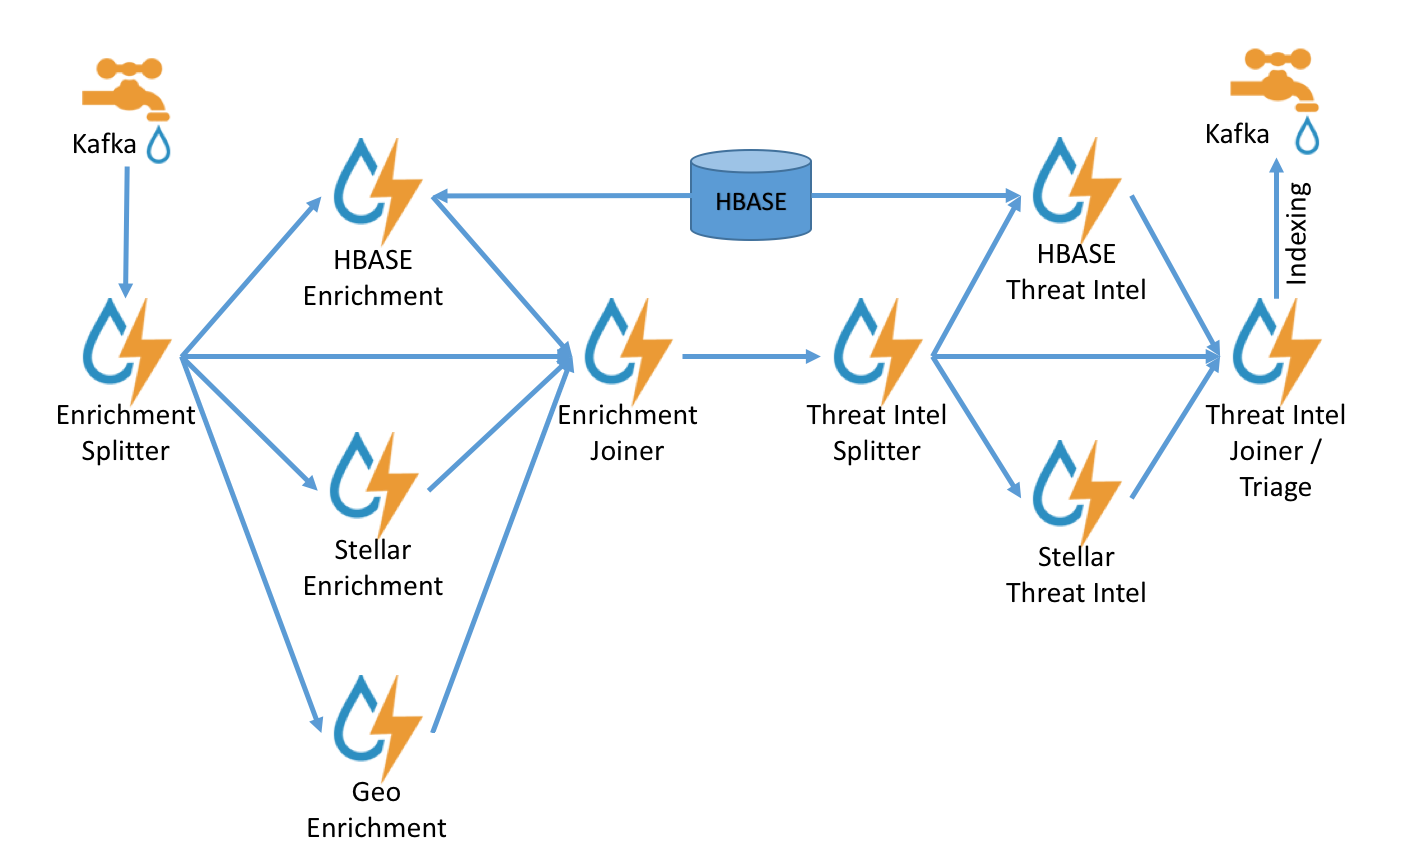
\includegraphics[scale=0.35]{images/enrichment_arch.png}}
\end{center}
}

\frame{\frametitle{Indexing}
\begin{center}
  \makebox[\textwidth]{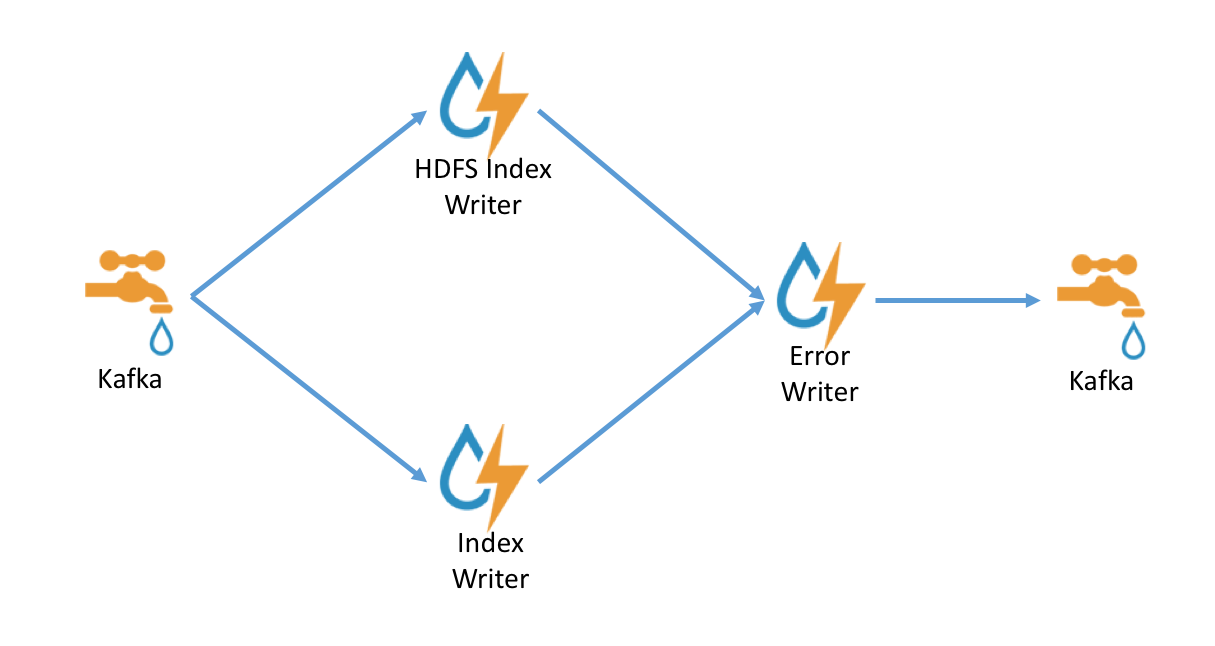
\includegraphics[scale=0.4]{images/indexing_arch.png}}
\end{center}
}

\frame{\frametitle{Profiler: Motivation}
\begin{itemize}
\item Enrichments and parsers operate within the context of a single message.  
\item This is insufficient for a number of scenarios
  \begin{itemize}
  \item Correlating between different sources
  \item Making judgments based on past events
  \item Both at the same time
  \end{itemize}
\item Operating across multiple sources has scalability implications
\item Waiting on the data you want from the other stream isn't plausible
\end{itemize}
}

\frame{\frametitle{Profiler: Solution}
\begin{itemize}
\item Compromise: Operate on windows in time rather than individual records
\item Windows should be able to be specified very flexibly to avoid seasonal aberrations.
\item The Profiler is a storm topology that takes the enriched data
  \begin{itemize}
  \item Capture aggregations of data in a window to HBase
  \item Uses Stellar to define how to aggregate data
  \item Uses Stellar to define a filter on which messages to consider
  \end{itemize}
\item These aggregations can be read anywhere Stellar is used
\item This enables things like
  \begin{itemize}
  \item Temporal outlier detection
  \item Limited context from other sources when building threat triage rules
  \end{itemize}
\end{itemize}
}

\frame{\frametitle{Profiler: Aggregations}
\begin{itemize}
\item Example aggregations:
  \begin{itemize}
  \item Distributional statistics: median, mean, percentile
  \item Set operations: Contains, Cardinality
  \item Simple counts
  \end{itemize}
\item Aggregations challenges
  \begin{itemize}
  \item May be big objects if naively done (e.g. set operations)
  \item May not be able to be merged across time (e.g. distributions)
  \item Profile reading should be decoupled from writing
  \end{itemize}
\item Approach: Use approximate data structures
  \begin{itemize}
  \item Set operations: Bloom Filters, HyperLogLog approximations
  \item Distributional Statistics: t-digests
  \end{itemize}
\end{itemize}
}

\frame{\frametitle{Demo}
\begin{itemize}
\item Los Alamos National Lab released an open data set representing 58 consecutive days of de-identified event data collected from five sources within Los Alamos National Laboratory's corporate, internal computer network.
\item Among other telemetry sources, authentication logs and a set of well-defined red teaming events that present bad behavior within the 58 days are provided.
\item We will look at the authentication logs around a breach and show how we can use Metron to pick out offending user's activity leading up to the event
  \begin{itemize}
  \item Look for users who are attempting to authenticate to many distinct hosts more than 5 standard deviations from the median across all users.
  \end{itemize}
\end{itemize}
}

\begin{frame}[fragile]
\begin{verbatim}
"profile": "distinct_auth_attempts_by_user",
"foreach": "user",
"onlyif": "source.type == 'auth'",
"init" : {
  "total" : "HLLP_INIT(5,6)"
         },
"update": {
  "total" : "HLLP_ADD(total, ip_dst_addr)"
          },
"result" : {
   "profile" : "total",
   "triage" : {
       "total_count" : "HLLP_CARDINALITY(total)"
              }
}
\end{verbatim}
\end{frame}

\begin{frame}[fragile]
\begin{verbatim}
"profile": "auth_distribution",
"foreach": "'global'",
"onlyif": "source.type == 'profiler' && profile == 'distinct_auth_attempts_by_user'",
"init" : {
  "s" : "STATS_INIT()"
         },
"update": {
  "s" : "STATS_ADD(s, total_count)"
          },
"result": "s"
\end{verbatim}
\end{frame}

\begin{frame}[fragile]
\begin{verbatim}
window := PROFILE_WINDOW('...')
profile := PROFILE_GET('distinct_auth_attempts_by_user', user, window)
distinct_auth_attempts := HLLP_CARDINALITY(GET_LAST(profile))
distribution_profile := PROFILE_GET('auth_distribution', 'global', window)
stats := STATS_MERGE(distribution_profile)
distinct_auth_attempts_median := STATS_PERCENTILE(stats, 0.5)
distinct_auth_attempts_stddev := STATS_SD(stats)
\end{verbatim}
\end{frame}

\frame{\frametitle{Questions}
Thanks for your attention!  Questions? 
\begin{itemize}
\item Find me at http://caseystella.com 
\item Twitter handle: @casey\_stella 
\item Email address: cstella@hortonworks.com
\end{itemize}
}

\end{document}
